\documentclass[english, aspectratio=169]{beamer}
% english is for the language used in standard texts (figures, tables etc)
% aspectratio of 16:9 or set it for more old school to 4:3 (without the ':')

% ---------------------------------------------------------------------------- %
% Load base preamble
% ---------------------------------------------------------------------------- %
\usepackage{import}
\subimport{./preamble/}{beamer.tex}

% ---------------------------------------------------------------------------- %
% Local macros
% ---------------------------------------------------------------------------- %

\newcommand{\Gvar}{\ensuremath{\calG_{\mathrm{var}}}}
\newcommand{\Gmul}{\ensuremath{\calG_{\mathrm{mul}}}}
\newcommand{\Gpoly}{\ensuremath{\calG_{\mathrm{poly}}}}
\newcommand{\GS}{\ensuremath{\calG(\calS)}}
\newcommand{\Gchance}{\ensuremath{\calG_{\mathrm{chance}}}}
\newcommand{\GexistsNE}{\ensuremath{\calG_{\exists \mathrm{NE}}}}
\newcommand{\GnoNE}{\ensuremath{\calG_{\mathrm{no NE}}}}
\newcommand{\Gpart}{\ensuremath{\calG_{\PARTITION}}}

\newcommand{\cHomQuad}{\cCLASS{HomQuad}}

% ------------------------------------------------------------------------------
% TITLEPAGE
% ------------------------------------------------------------------------------
\title{
  \cETR-completeness of Nash equilibria in Perfect Information Stochastic
  Games
}

\author{Kristoffer Arnsfelt Hansen and \textbf{Steffan S\o lvsten}}

\date{August 2020}

\institute{
\includegraphics[width=0.2\linewidth]{./external/aulogo_uk_var2_black.eps}}

\begin{document}

\titleframe

\begin{frame}[plain,noframenumbering]{}
  \tableofcontents
\end{frame}

\section{Stochastic Games}
\subsection{Basic definitions and utility functions}

\begin{frame}
  \frametitle{Stochastic Games}

  \begin{columns}
    \begin{column}{0.5\textwidth}
      An $m$-player perfect information stochastic game $G$ is defined by
      \begin{itemize}
        \onslide<2-> {
        \item Directed graph $(V, A)$ }

        \onslide<3-> {
        \item An initial node $v_o \in V$. }

        \onslide<4-> {
        \item $V$ is partitioned into disjoint sets $V_0, V_1, \dots, V_m$, where
          $V_i$ are controlled by Player~$i$ and $V_0$ are \emph{chance} nodes. }
      \end{itemize}

      
      \onslide<2-> {
        \begin{tikzpicture}[thick, minimum size = 0.8cm]
          \node[shape=circle, draw=black] (v3) {};
          \onslide<2-3>{
            \node[shape=circle, draw=black, left=of v3] (v2) {};
          }
          \node[shape=circle, draw=black, left=of v2] (v1) {};

          \onslide<3-> {
            \node[draw=none, left=-.2cm of v1] (v1_i) {$\rightarrow$};
          }

          \onslide<4-> {
            \node[shape=diamond, minimum size = 1cm, draw=black, left=0.9cm of v3] (v2_c) {};
            
            \node[draw=none, above=-.2cm of v1] (v1_i) {$1$};
            \node[draw=none, above=-.2cm of v3] (v1_i) {$2$};
          }
          
          \path[->]
          (v1) edge[bend right] (v2)
          (v3) edge[bend left] (v2)
          (v2) edge[bend left] (v3)
          (v2) edge[bend right] (v1)
          ;
        \end{tikzpicture}        
      }
    \end{column}
    \begin{column}{0.5\textwidth}
      \begin{itemize}
        \onslide<5->{
        \item A play $h \in \calH_\infty$ is an infinite sequence $(h_t)_{t \geq
            0}$ of vertices in $V$, where

          \begin{equation*}
            h_0 = v_0,
            \quad
            (h_t, h_{t+1}) \in A
          \end{equation*}
        }

        \onslide<6->{
        \item Utility functions $u_i$ assigns a payoff $u_i(i)$ for Player~$i$
          to a play $h \in \calH_\infty$}
      \end{itemize}
    \end{column}
  \end{columns}
\end{frame}

\begin{frame}
  \frametitle{Mean-payoff games}

  \begin{figure}
    \centering

    \begin{tikzpicture}[thick, minimum size = 0.8cm]
      \node[shape=circle, draw=black, label=above:$1$, label=left:$\rightarrow$] (v1) {};

      \node[shape=circle, draw=black, label=above:$2$, above right=1cm and 2cm of v1] (v2) {};
      \node[shape=circle, draw=black, label=above:$2$, right=2cm of v2] (v2_2) {};
      \node[shape=circle, draw=black, label=above:$3$, below right=1cm and 2cm of v1] (v3) {};

      \path[->]
        (v1) edge[bend left=30]  node[above] {$1,0,0$} (v2)
        (v2) edge[bend left=10]  node[above] {$0,1,0$} (v2_2)
        (v2_2) edge[bend left=10] node[below] {$1,1,0$} (v2)
        (v1) edge[bend right=30] node[below] {$0,0,0$} (v3)
        (v3) edge[loop right] node[right] {$1,0,1$} ()
      ;

      \path[<->] (v2) edge[bend left=30] node[right] {$0,1,1$} (v3);

      \onslide<2-2> {
        \path[->, very thick, cyan]
          (v1) edge[bend right=30] (v3)
          (v3) edge[loop right] ()
        ;
      }

      \onslide<3-3> {
        \path[->, very thick, cyan]
          (v1) edge[bend left=30] (v2)
          (v2) edge[bend left=10] (v2_2)
          (v2_2) edge[bend left=10] (v2)
        ;
      }

      \onslide<4-4> {
        \path[->, very thick, cyan]
          (v1) edge[bend left=30] (v2)
        ;
        \path[<->, very thick, cyan] (v2) edge[bend left=30] (v3);
      }
    \end{tikzpicture}
    
    \caption{A simple mean-payoff game.
      \onslide<2-4>{Mean payoff for player $1$: \temporal<3>{$1$}{$\tfrac{1}{2}$}{$0$}}
    }
    \label{fig:mean-payoff game}
  \end{figure}
\end{frame}

\begin{frame}
  \frametitle{Recursive games}

  \begin{figure}
    \centering

    \begin{tikzpicture}[thick, minimum size = 0.8cm]
      \node[shape=circle, draw=black, label=above:$1$, label=left:$\rightarrow$] (v1) {};
      \node[shape=diamond, draw=black, right=2cm of v1] (chance) {};
      \node[shape=circle, draw=black, label=above:$2$, right=2cm of chance] (v2) {};

      \path[->]
        (v1) edge[bend right] (chance)
        (v2) edge[bend left] (chance)
        (chance) edge[bend left] node[above left=-0.2cm and 0.3cm] {$\tfrac{1}{4}$} (v2)
        (chance) edge[bend right] node[above right=-0.2cm and 0.3cm] {$\tfrac{1}{4}$} (v1)
      ;
      
      \onslide<1-1>{
        \node[shape=circle, draw=black, below=of v1] (payoff_v1) {};
        \node[shape=circle, draw=black, below=of chance] (payoff_chance) {};
        \node[shape=circle, draw=black, below=of v2] (payoff_v2) {};

        \path[->]
          (v1) edge (payoff_v1)
          (chance) edge (payoff_chance)
          (v2) edge (payoff_v2)
          (payoff_v1) edge[loop below] node[below] {$0,1$} ()
          (payoff_chance) edge[loop below] node[below] {$\tfrac{1}{2} , \tfrac{1}{2}$} ()
          (payoff_v2) edge[loop below] node[below] {$\tfrac{1}{2} , \tfrac{1}{2}$} ()          
        ;
      }

      \onslide<2-2>{
        \node[below=of v1] (payoff_v1) {$(0 , 1)$};
        \node[below=of chance] (payoff_chance) {$(\tfrac{1}{2} , \tfrac{1}{2})$};
        \node[below=of v2] (payoff_v2) {$(1 , 0)$};

        \path[->]
          (v1) edge (payoff_v1)
          (chance) edge (payoff_chance)
          (v2) edge (payoff_v2)
        ;
      }
    \end{tikzpicture}
    
    \caption{A simple game with terminal rewards only. Ummels '11}
    \label{fig:terminal rewards}
  \end{figure}
\end{frame}

\subsection{Nash Equilibria}
\begin{frame}
  \frametitle{Strategies and Nash equilibria}
  A strategy $\tau_i$ assigns a probability distribution to the outgoing arcs of
  vertices $v \in V_i$ depending on the given history $h$.

  \begin{itemize}
  \item A strategy is \emph{stationary}, if the choice of the players at a
    vertice is independent of the prior history of play (i.e. the strategy is
    memoryless).
  \end{itemize}
  
  \pause
  
  We assume players are acting \emph{rationally}. This is commonly captured by
  the following notion

  \begin{definition}[Nash equilibria]
    A strategy profile $\tau = (\tau_1, \tau_2, \dots, \tau_m)$ is a \emph{Nash
      equilibrium}, if no player $i$ has a unilateral deviation available that
    strictly improves their payoff.
  \end{definition}
\end{frame}

\begin{frame}
  \frametitle{Subgame Perfect Nash equilibria}
  \begin{figure}
    \centering

    \begin{tikzpicture}[thick, minimum size = 0.8cm]
      % Nodes
      \node[shape=circle, draw=black, label=above:$1$, label=left:$\rightarrow$] (v1) {$v_1$};
      \node[shape=circle, draw=black, label=above:$2$, right=2cm of v1] (v2) {$v_2$};

      % Payoffs
      \node[draw=none, below =.5cm of v1]    (payoff1)   {$(0,0)$};
      \node[draw=none, below =.5cm of v2]    (payoff2_1) {$(0,0)$};
      \node[draw=none, right =1.4cm of v2] (payoff2_2) {$(1,1)$};

      \path[->]
      (v1) edge (v2)
        (v1) edge (payoff1)
        (v2) edge (payoff2_1)
        (v2) edge (payoff2_2)
      ;

      
      % Sensible equilibria
      \onslide<2-2,5-5>{
        \path[->, very thick, cyan]
          (v1) edge (v2)
          (v2) edge (payoff2_2)
        ;        
      }

      % Irrational equilibria
      \onslide<3-4>{
        \path[->, very thick, cyan]
          (v1) edge (payoff1)
          (v2) edge (payoff2_1)
        ;        
      }
    \end{tikzpicture}
    
    \caption[Irrational Nash equilibria]{A two-player reachability game with an
      irrational Nash equilibrium. Ummels '11}
    \label{fig:irrational Nash equilibria}
  \end{figure}

  \onslide<4->{
    \begin{definition}[Subgame Perfect Nash equilibria]
      A \emph{Subgame perfect} Nash equilibrium is a NE of a game $G$, that is
      \emph{not} only the best response from $v_0$, but is a best response in
      $G[h]$ given \emph{any} history $h$ of play.
    \end{definition}
  }
\end{frame}

\subsection{Game Theory in Model Checking and Synthesis}
\begin{frame}
  \frametitle{Game Theory in Model Checking}
  Games provide a well studied framework that can capture many model checking
  problems with \emph{adversaries}.
  \begin{itemize}
  \item A protocol between $m$ entities can be described by a stochastic game of
    $m$ players.
  \item A distributed system of $m$ peers can be described by a
    \emph{concurrent} game of $m$ players.
  \end{itemize}

  \vspace{6pt} \pause Classical model checking objectives can be encapsulated in
  the utility function.
  \begin{itemize}
  \item \emph{Reachability} objectives can be captured by payoffs in $\{ 0,1 \}$
    in a recursive game.
  \item \emph{Safety} objectives can be captured by payoffs in $\{ -1, 1 \}$ in
    a recursive game, since an \emph{infinite} game has payoff $0$.
  \item Other Büchi objectives can also be described in general Mean-payoff games.
  \end{itemize}
\end{frame}

\begin{frame}
  \frametitle{Game Theory in Synthesis}

  The problem of \emph{synthesis} is to not only check a program satisfies a
  given specification, but to also generate parts of the program according to
  the specification.

  \begin{center}
    Does there exist a controller, such that the system satisfies the
    specification?

    \pause
    \vspace{10pt} $\equiv$ \vspace{10pt}

    Does there exist a strategy, such that Player~$1$ is surely winning?
  \end{center}
\end{frame}

\begin{frame}
  \frametitle{The subject of this seminar}

  Consider the problem:

  \vspace{10pt}
  
  \begin{center}
    Given an $m$-player game G and payoff demands $L \in \R^m$, \\
    does there exist a stationary \footnote{ The problem of existence of a Nash
      equilibria satisfying some demands is undecidable for $\geq 10$ players in
      recursive games, so we will only focus on \emph{stationary} strategies. }
    NE $\tau$ with $U(\tau) \geq L$?
  \end{center}

  We will show this is \cETR-complete.
\end{frame}

\section{\cETR-complexity}

\begin{frame}
  \frametitle{\cETR\ Complexity Class}
  \vspace{-25pt}
  \begin{figure}
    \centering

    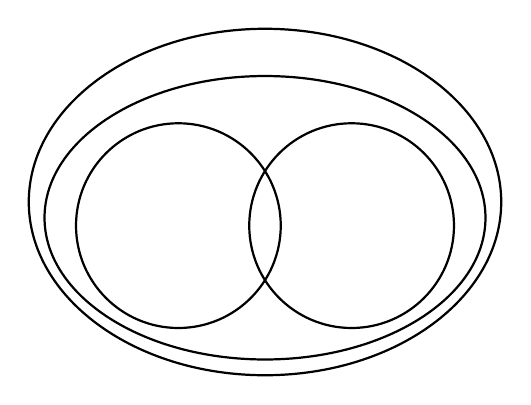
\begin{tikzpicture}[thick]
      \onslide<1->{
        \draw (-1.1,-.3) circle (1.3cm) node {\cNP};
        \draw (1.1,-.3) circle (1.3cm) node {\cSqrtSum};
      }

      \onslide<2->{
        \draw (0,-.2) ellipse (2.8cm and 1.8cm) node[above=1cm] {\cETR};;
      }

      \onslide<3->{
        \draw (0,0) ellipse (3cm and 2.2cm) node[above=1.6cm] {\cPSPACE};;
      }      
    \end{tikzpicture}
    
    \caption{The relation between \cNP, \cSqrtSum, and \cETR}
    \label{fig:complexity classes related}
  \end{figure}
  \onslide<2-> {
    \vspace{-15pt}
    The complexity class \cETR\ both encapsulates the hardness of \cNP\ decision
    problems and the hardness of computing with real numbers of \cSqrtSum.
  }
\end{frame}

\subsection{The \cNP\ and \cSqrtSum\ Complexity Classes}
\begin{frame}
  \frametitle{\cNP\ Complexity Class}

  Remember that the well-known class \cNP can be captured by the \cILP\ problem:
  \begin{align*}
    \min \quad  &c^T x
    \\
    \text{s.t.} \quad
                &Ax \leq b
    \\
                &x \in \N^n
  \end{align*}
  where $A \in \Z^{n \times m}$, $b \in \Z^m$, $c \in \Z^n$
\end{frame}

\begin{frame}
  \frametitle{\cSqrtSum\ Complexity Class}

  Consider the following problem: Given $a_1, a_2, \dots a_n, b_1, b_2, \dots,
  b_m \in \R$ is the following inequality satisfied?
  \begin{equation*}
    \sum_{i=1}^n \sqrt{a_i} \leq \sum_{j=1}^m \sqrt{b_j}
  \end{equation*}

  Seems trivial... \pause How many decimals do you have to compute, before you
  know the answer? \footnotemark

  \footnotetext[1]<2->{This consistently comes up in Computational Geometry.
    Here, theoretical works solve this by assuming the $\R$-RAM computational
    model; leaving an adventure for implementors to experience later.}

  \begin{definition}[\cSqrtSum]
    The complexity class \cSqrtSum\ consists of all problems that are polynomial
    time reducible to the problem above.
  \end{definition}
\end{frame}


\subsection{The \cETR\ Complexity Class}
\begin{frame}
  \frametitle{\cETR\ Complexity Class}

  The \emph{Existential Theory of the Reals} is the language of all true
  sentences of the form
  \begin{equation*}
    \exists x_1, x_2, \dots, x_n \in \R : \phi(x_1, x_2, \dots, x_n)
  \end{equation*}
  where $\phi$ is a quantifier-free Boolean formula of inequalities and
  equalities.

  \pause
  \begin{definition}[\cETR]
    The complexity class \cETR\ consists of all problems, that are polynomial
    time reducible to the existential theory of the reals.
  \end{definition}
\end{frame}

\begin{frame}
  \frametitle{\cETR\ Complexity Class}
  
  We will consider the following \cETR-complete problem.

  \begin{definition}[\cHomQuad]
    Given a system \calS\ of $l$ \emph{homogeneous quadratic} polynomials
    \footnote{ A homogenous quadratic polynomial is of the form $\sum_{i = 1}^n
      \sum_{j=1}^n A_{ij} x_{i} x_{j}$ where $A \in [ -1,1 ]^{n \times n}$.}
    in $n$ variables, does there exist an $x \in \R^n$ such that $q_k(x) = 0$
    for all $k \in \{1, 2, \dots, l\}$ and $x$ is a probability distribution?
  \end{definition}

\end{frame}

\section{Proof Sketch: \cETR-Completeness of Nash equilibria}

\begin{frame}
  \frametitle{\cETR-Completness of Nash equilibria}

  Consider the problem:

  \vspace{10pt}
  
  \begin{center}
    Given an $m$-player game G and payoff demands $L \in \R^m$, \\
    does there exist a stationary NE $\tau$ with $U(\tau) \geq L$?
  \end{center}

  \pause \vspace{10pt}

  It has already been shown to be \cNP-hard for $\geq 2$ players and
  \cSqrtSum-hard for $\geq 4$ players. Furthermore, it is contained within
  \cETR.
\end{frame}

\begin{frame}
  It is \cETR-complete! We will show this by reduction to:

  \begin{definition}[\cHomQuad]
    Given a system \calS\ of $l$ \emph{homogeneous quadratic} polynomials in $n$
    variables, does there exist an $x \in \R^n$ such that $q_k(x) = 0$ and $x$
    is a probability distribution?
  \end{definition}

  \pause \vspace{15pt}
  That is, given a system \calS\ of $l$ polynomials of the form
  \begin{equation*}
    q_k(x) = a_{1,1} x_1 x_1 + a_{1,2} x_1 x_2 + \dots + a_{ij} x_i x_j + \dots a_{n n} x_n x_n
  \end{equation*}
  we will construct a game $\calG(\calS)$ such that all $q_k(x) = 0$ if and only
  if $\calG(\calS)$ has a stationary Nash equilibria that satisfies some payoff
  demand.
\end{frame}

\subsection{Gadgets}
\begin{frame}
  \frametitle{Proof Sketch: $\Gvar$}

  \begin{columns}
    \begin{column}{0.6\textwidth}
      \begin{figure}
        \centering

        \begin{tikzpicture}[thick, shorten >= 1, node distance = 2cm, on grid, minimum size = 0.8cm]
          \node[shape=diamond, draw=black, label=left:$\rightarrow$] (e1) {};
          % HACK: Moves - - -> arrow head to the left
          \node[draw=none] (n1_i) [right=of e1] {\phantom{MM}};
          \node[shape=circle, draw=black, label=above:$1$] (n1_1) [above=1.5cm of n1_i] {$v_1$};
          \node[draw=none] (g1_1) [above right=0.4cm and 3cm of n1_1] {$(0,1,0,1,0,0,0)$};
          \node[draw=none] (g1_2) [below right=0.4cm and 3cm of n1_1] {$(0,0,1,0,1,0,0)$};
          \node[shape=circle, draw=black, label=above:$1$] (n1_n) [below=1.5cm of n1_i] {$v_n$};
          \node[draw=none] (gn_1) [above right=0.4cm and 3cm of n1_n] {$(0,1,0,1,0,0,0)$};
          \node[draw=none] (gn_2) [below right=0.4cm and 3cm of n1_n] {$(0,0,1,0,1,0,0)$};
          \path[->]
             (e1) edge [bend left=10] node [above left] {$\frac{1}{n}$} (n1_1)
                  edge [bend right=10] node [below left] {$\frac{1}{n}$} (n1_n)
             (n1_1) edge [bend left=8] node [above] {\small \color{gray} $x_1$} (g1_1)
                    edge [bend right=8] (g1_2)
             (n1_n) edge [bend left=8] node [above] {\small \color{gray} $x_n$} (gn_1)
                    edge [bend right=8] (gn_2)
           ;
           \path[->] (e1) edge (n1_i) [loosely dashed];
           % vertical dots between n1_1 and n1_n
           \path (n1_1) edge node [black, opacity=1, sloped] {\dots} (n1_n) [opacity=0];
        \end{tikzpicture}
        
        \caption{The gadget game $\Gvar$}
        \label{fig:Gvar}
      \end{figure}
    \end{column}
    \begin{column}{0.4\textwidth}
      At each $v_i$, Player~$1$ can choose to either give payoff $1$ to players
      $2$ and $4$ or $3$ and 5.

      \pause \vspace{10pt}
      Player~$1$ strategy corresponds to a probability distribution if it
      satisfies the payoff demand
      \begin{equation*}
        \left(
          0,
          \frac{1}{n},
          \frac{n-1}{n},
          \dots
        \right)
      \end{equation*}
    \end{column}
  \end{columns}
\end{frame}

\begin{frame}
  \frametitle{Proof Sketch: $\Gmul(i,j,\alpha)$}

  \begin{figure}
    \centering

    \begin{tikzpicture}[thick, shorten >= 1, node distance = 2cm, on grid, minimum size = 0.8cm]
        % First threat
      \node[shape=circle, draw=black]
          (threat1) {$v_i$};
      \node[shape=circle, draw=black, label=above:$2$, label=left:$\rightarrow$]
          (threat1_1) [above left=1.4cm and 0.6cm of threat1] {$w_1$};
      \node[shape=circle, draw=black, label=above:$3$]
          (threat1_2) [above right=1.4cm and 0.6cm of threat1] {$w_2$};
      % Replication of x_i
      \node[shape=circle, draw=black, label=above:$1$]
          (repl1) [right=1.7cm of threat1_2] {$w_3$};
      \node[draw=none]
          (repl1_terminal) [below=1.4cm of repl1] {$(1,0,1,0,0,0,0)$};

      \onslide<1-1>{
        \node[shape=circle, draw=none] (threat2_1_dummy) [right=1.7cm of repl1] {$\cdots$};
      }

      \path[->]
          (threat1_1) edge [bend left=5] (threat1)
          (threat1_1) edge (threat1_2)
          (threat1_2) edge [bend right=5] (threat1)
          (threat1_2) edge (repl1)

          (repl1) edge node [above=-0.15cm] {\small \color{gray} $x_i'$} (threat2_1_dummy)
                  edge node [right] {\small \color{gray} $1-x_i'$} (repl1_terminal)
      ;
          
      \onslide<2-2> {
        % Second threat
        \node[shape=circle, draw=black, label=above:$4$]
            (threat2_1) [right=1.7cm of repl1] {$w_4$};
        \node[shape=circle, draw=black, label=above:$5$]
            (threat2_2) [right=1.2 of threat2_1] {$w_5$};
        \node[shape=circle, draw=black]
            (threat2) [below right=1.4cm and 0.6cm of threat2_1] {$v_j$};
        % Replication of x_i
        \node[shape=circle, draw=black, label=above:$1$]
            (repl2) [right=1.7cm of threat2_2] {$w_6$};
        \node[draw=none] (repl2_terminal1)
            [above right=1.5cm and 1.5cm of repl2] {$(1,1,0,1,0,\alpha,1-\alpha)$};
        \node[draw=none] (repl2_terminal2)
            [below right=1.5cm and 1.5cm of repl2] {$(1,1,0,0,1,0,0)$};
        \path[->]
            (threat2_1) edge (threat2_2)
            (threat2_1) edge [bend left=5] (threat2)
            (threat2_2) edge [bend right=5] (threat2)
            (threat2_2) edge (repl2)
            (repl2) edge [bend right=10]
                    node [right=.2cm] {\small \color{gray} $x_j'$} (repl2_terminal1)
            (repl2) edge [bend left=10]
                    node [right=.2cm] {\small \color{gray} $1 - x_j'$} (repl2_terminal2)
        ;
      }
    \end{tikzpicture}

    \caption{The gadget game $\Gmul(i,j,\alpha)$}
    \label{fig:Gmul}
  \end{figure}

  \onslide<2->{
    If Player~$1$ receives payoff $1$, then Player-$6$ gets $\alpha x_i x_j$ and
    Player-$7$ gets $(1-\alpha) x_i x_j$.
  }
\end{frame}

\begin{frame}
	\begin{equation*}
		\max {}_{\tau_1}
		\min {}_{\tau_2}
	 	\Pr \left[ u_1(v_0(\tau_1, \tau_2)) = 1 \right]
	\end{equation*}
	
	\begin{equation*}
		\forall \tau_2 : \Pr \left[ u_1(v_0(\tau_1,\tau_2)) = 1 \right] \geq \text{value}
	\end{equation*}
\end{frame}

\begin{frame}
  \frametitle{Proof Sketch: $\Gpoly(q)$}
  
  For a homogenous quadratic polynomial $q_k(x) = \sum_{i,j=1}^n A_{ij} x_i x_j$.

  \begin{figure}
    \centering

    \begin{tikzpicture}[thick, shorten >= 1, node distance = 2cm, on grid, minimum size = 0.8cm]
      % Threats
      \node[shape=circle, draw=black, label=above:$6$, label=left:$\rightarrow$] (threat1) {};
      \node[draw=none] (threat1_t) [below=1.3cm of threat1] {$(0,0,0,0,0,\frac{1}{2 n^2},0)$};
      \node[shape=circle, draw=black, label=above:$7$] (threat2) [right=3.3cm of threat1] {};
      \node[draw=none] (threat2_t) [below=1.3cm of threat2] {$(0,0,0,0,0,0,\frac{1}{2n^2})$};
      % Chance node
      \node[shape=diamond, draw=black] (chance_node) [right=2cm of threat2] {};
      % Subgames
      \node[draw=none] (g1_1) [above right=1.2cm and 3cm of chance_node] {$\Gmul(x_1,x_1,\frac{1 + A_{1 1}}{2})$};
      \node[draw=none] (gi_j) [above right=0cm and 3cm of chance_node] {$\Gmul(x_i,x_j,\frac{1 + A_{i j}}{2})$};
      \node[draw=none] (gn_n) [below right=1.2cm and 3cm of chance_node] {$\Gmul(x_n,x_n,\frac{1 + A_{n n}}{2})$};
      % HACK: Nodes for dashed arrows
      \node[draw=none] (gi) [below right=0.6cm and 2cm of chance_node] {};
      \node[draw=none] (gj) [above right=0.6cm and 2cm of chance_node] {};
      % Edges
      \path[->]
        (threat1) edge (threat2)
        (threat1) edge (threat1_t)
        (threat2) edge (threat2_t)
        (threat2) edge (chance_node)
        (chance_node) edge [bend left=20] node [left] {$\frac{1}{n^2}$} (g1_1)
        (chance_node) edge (gi_j)
        (chance_node) edge [bend right=25] node [left] {$\frac{1}{n^2}$} (gn_n)
      ;
      \path[->]
        (chance_node) edge [bend right=10] (gi)
        (chance_node) edge [bend left=10] (gj)[loosely dashed]
      ;
      % Dots
      \path[-]
        (g1_1) edge (gi_j)
        (gi_j) edge (gn_n) [loosely dotted, thick]
      ;
    \end{tikzpicture}
    
    \caption{The gadget game $\Gpoly(q_k)$}
    \label{fig:Gpoly}
  \end{figure}

  If Player~$1$ receives payoff $1$, then Player~$6$ gains payoff
  $\frac{1}{2n^2} (\norm{x}^2_1 + q_k(x))$.

  If also $\norm{x}_1$ is $1$, then $q_k(x) = 0$.
\end{frame}

\subsection{Reduction}
\begin{frame}
  \frametitle{Proof Sketch: Final reduction}

  \begin{columns}
    \begin{column}{0.6\textwidth}
      \begin{figure}
        \centering

        \begin{tikzpicture}[thick, shorten >= 1, node distance = 2cm, on grid, minimum size = 0.8cm]
          % Leftmost chance node
          \node[shape=diamond, draw=black, label=left:$\rightarrow$] (e1) {$v_0$};
          % G1(n)
          \node[draw=none] (G1) [above right=1cm and 2cm of e1] {$\Gvar$};
          % Choice of polynomia
          \node[shape=diamond, draw=black] (e2) [below right=1cm and 2cm of e1] {};
          \node[draw=none] (q1) [above right=0.8cm and 2cm of e2] {$\Gpoly(q_1)$};
          \node[draw=none] (qi) [right=of e2] {\phantom{MM}};
          \node[draw=none] (qn) [below right=0.8cm and 2cm of e2] {$\Gpoly(q_\ell)$};

          \path[->]
            (e1) edge [bend left=25] node [above left=-0.2cm] {$\frac{1}{2}$} (G1)
            (e1) edge [bend right=25] node [below left=-0.2cm] {$\frac{1}{2}$} (e2)
            (e2) edge [bend left=25] node [above left=-0.2cm] {$\frac{1}{\ell}$} (q1)
            (e2) edge [bend right=25] node [below left=-0.2cm] {$\frac{1}{\ell}$} (qn)
          ;
          \path[->] (e2) edge (qi) [loosely dashed];
          % vertical dots between q1 and qn
          \path (q1) edge node [black, opacity=1, sloped] {\dots} (qn) [opacity=0];
        \end{tikzpicture}
        
        \caption{The game $\calG(\calS)$ of the reduction}
        \label{fig:G}
      \end{figure}    
    \end{column}
    \begin{column}{0.4\textwidth}
      $\calS$ is a ``yes''-instance of \cHomQuad\ if and only if the game
      $\calG(\calS)$ has a Nash Equilibria that satisfies the demands
      \begin{equation*}
        \left(
          \frac{1}{2},
          \frac{1}{n},
          \frac{n-1}{n},
          0,
          0,
          \dots,
          0
        \right)
      \end{equation*}
    \end{column}
  \end{columns}
\end{frame}

\begin{frame}
  \begin{theorem}
    It is $\cETR$-complete to decide whether for a given $m$-player
    recursive game $G$ and payoff demands $L \in \R^m$ there exists a
    stationary Nash equilibria $\tau$ with $U(\tau)\geq L$.

    \begin{itemize}
    \item The problem is $\cETR$-complete even for acyclic $7$-player recursive
      games with non-negative rewards.
    \item It even holds for stationary Subgame Perfect Equilibria.
    \end{itemize}      
    \end{theorem}
\end{frame}

\section{Implications for Model Checking}
\begin{frame}
  \frametitle{\cETR-Completeness of Stationary NE without Payoff Demands}

  \begin{columns}
    \begin{column}{0.5\textwidth}

      \begin{figure}
        \centering

        \begin{tikzpicture}[thick, shorten >= 1, node distance = 2cm, on grid, minimum size = 0.8cm]
          % Threats
          \node[shape=circle, draw=black, label=above:$1$, label=left:$\rightarrow$]
              (threat1) {$t_1$};
          \node[shape=circle, draw=black, label=above:$2$]
              (threat2) [right  = 1.6cm of threat1] {$t_2$};
          \node[shape=circle, draw=black, label=above:$3$]
              (threat3) [right  = 1.6cm of threat2] {$t_3$};

          % Chance node
          \node[shape=diamond, draw=black] (chance) [below  = 2cm of threat2] {$t_4$};

          % Games
          \node[draw=none] (game_reduction) [right  = 2cm of threat3] {$\GS$};
          \node[draw=none] (game_no_NE) [left  = 1.7cm of chance] {$\GnoNE$};
          \node[draw=none] (chance_term) [right  = 2.8cm of chance]
            {$2 \cdot \left( \frac{1}{2}, \frac{1}{n}, \frac{n-1}{n}, 0, \dots, 0 \right)$};

          \draw[->]
            (threat1) edge (threat2)
                      edge [bend left=20] (chance)
            (threat2) edge (threat3)
                      edge (chance)
            (threat3) edge (game_reduction)
                      edge [bend right=20] (chance)
        
            (chance) edge node[below] {$\frac{1}{2}$} (game_no_NE)
                     edge node[below] {$\frac{1}{2}$} (chance_term)
          ;
        \end{tikzpicture}
        
        \caption{The game $\GexistsNE(\calS)$}
        \label{fig:GexistsNE}
      \end{figure}      
    \end{column}

    \begin{column}{0.05\textwidth}
    \end{column}
    
    \begin{column}{0.45\textwidth}
      $\GnoNE$ is an independent sub-game,
      \begin{itemize}
      \item Has \emph{no} stationary Nash equilibria
      \item Players $1$, $2$, $3$ always get payoff $0$.
      \end{itemize}

      \pause \vspace{10pt}

      $\calS$ is a ``yes''-instance of \cHomQuad\ if and only if the game
      $\GexistsNE(\calS)$ has a stationary Nash Equilibria.
    \end{column}
  \end{columns}
\end{frame}

\begin{frame}
  \frametitle{\cETR-Completeness of Reachability and Safety objectives}
  
  There exists different $\GnoNE$ gadget games for the different restrictions of
  the utility function:
  \begin{itemize}
  \item Reachability objective
  \item Safety objective
  \end{itemize}

  \vspace{20pt}
  
  \begin{theorem}
    It is $\cETR$-complete to decide whether a given $m$-player game with
    Reachability or Safety objectives has a stationary NE.
    \begin{itemize}
    \item even for $m = 7$ players.
    \end{itemize}
  \end{theorem}

\end{frame}

\begin{frame}
  \frametitle{\cETR-Completeness of being almost surely winning}

  Consider the game $\GexistsNE(\calS)$ in which another player is added, who is
  always winning in $\calG(\calS)$, but not in $\GnoNE$.

  \vspace{20pt}

  \begin{theorem}
    For any $i$, it is $\cETR$-complete to decide whether a given $m$-player
    recursive game has a stationary NE in which Player~$i$ is \emph{almost
      surely winning}.
    \begin{itemize}
    \item even for $m = 8$ players.
    \end{itemize}

  \end{theorem}  
\end{frame}

\begin{frame}
  \frametitle{Final remarks}

  It is \cETR-complete to decide in an $m$-player perfect information recursive
  game.
  \begin{itemize}
  \item exists Subgame Perfect Nash equilibria satisfying demand $L \in \R^m$
  \item exists any Nash equilibria for \emph{Reachability} and \emph{Safety} objectives
  \item exists any Nash equilibria such that Player~$1$ is surely winning.
  \end{itemize}

  \pause
  
  Notice here that
  \begin{itemize}
  \item This problem is already shown by Ummels '11 to be \cNP-hard for $\geq 2$
    players and \cSqrtSum-hard for $\geq 4$ players so this completeness result
    could not become much tighter.
    
  \item There have been recent results of \cETR-completeness in \emph{imperfect
      information} games. The complexity of these results stem from the
    structure of the game, not the lack of information.
  \end{itemize}
  
\end{frame}

\end{document}

%%% Local Variables:
%%% mode: latex
%%% TeX-master: t
%%% End:
